\section{Use Case Diagrams}
\label{sec:usecasediagrams}

This section outlines the use case diagrams for the product, which represent the user's interaction with 
the system. Standard UML notation is used. \cite{usecaseUML} There are 3 main elements involved in a use 
case diagram, the actor who interacts with the system, the use cases, that are tasks that can be performed 
by the system, and lines that represent dependencies among the use cases. The lines that are marked "include" 
are used to show the relationship between use cases where one can be reached from the other.

Figure \ref{fig:ucdmenu} shows the functionality provided by the application from a superior view of 
the game, while Figure \ref{fig:ucdgameplay} shows the functionality provided while in gameplay mode.

\begin{figure}[H]
  	\centering
	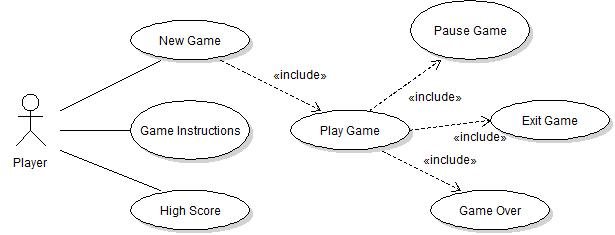
\includegraphics[width=\textwidth]{pictures/UCD_Game_Menu.jpg}
	\caption{Use Case Diagram of Game Menu}
	\label{fig:ucdmenu}
\end{figure}

\begin{figure}[H]
  	\centering
	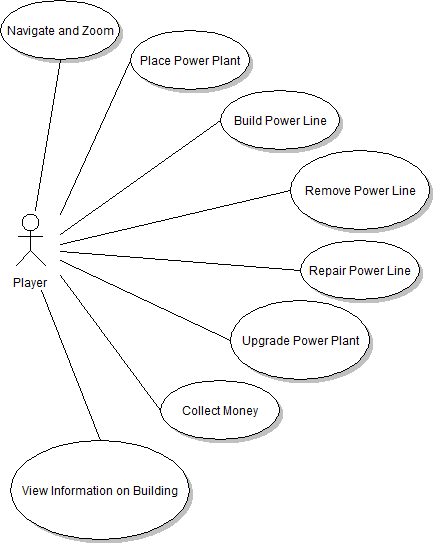
\includegraphics[width=\textwidth]{pictures/UCD_PlayGame.png}
	\caption{Use Case Diagram of Gameplay}
	\label{fig:ucdgameplay}
\end{figure}

